\chapter*{Appendix}
\addcontentsline{toc}{chapter}{Appendix}
\section{Trajectories of public datasets }
%\begin{figure}[h!]
%	\centering
%	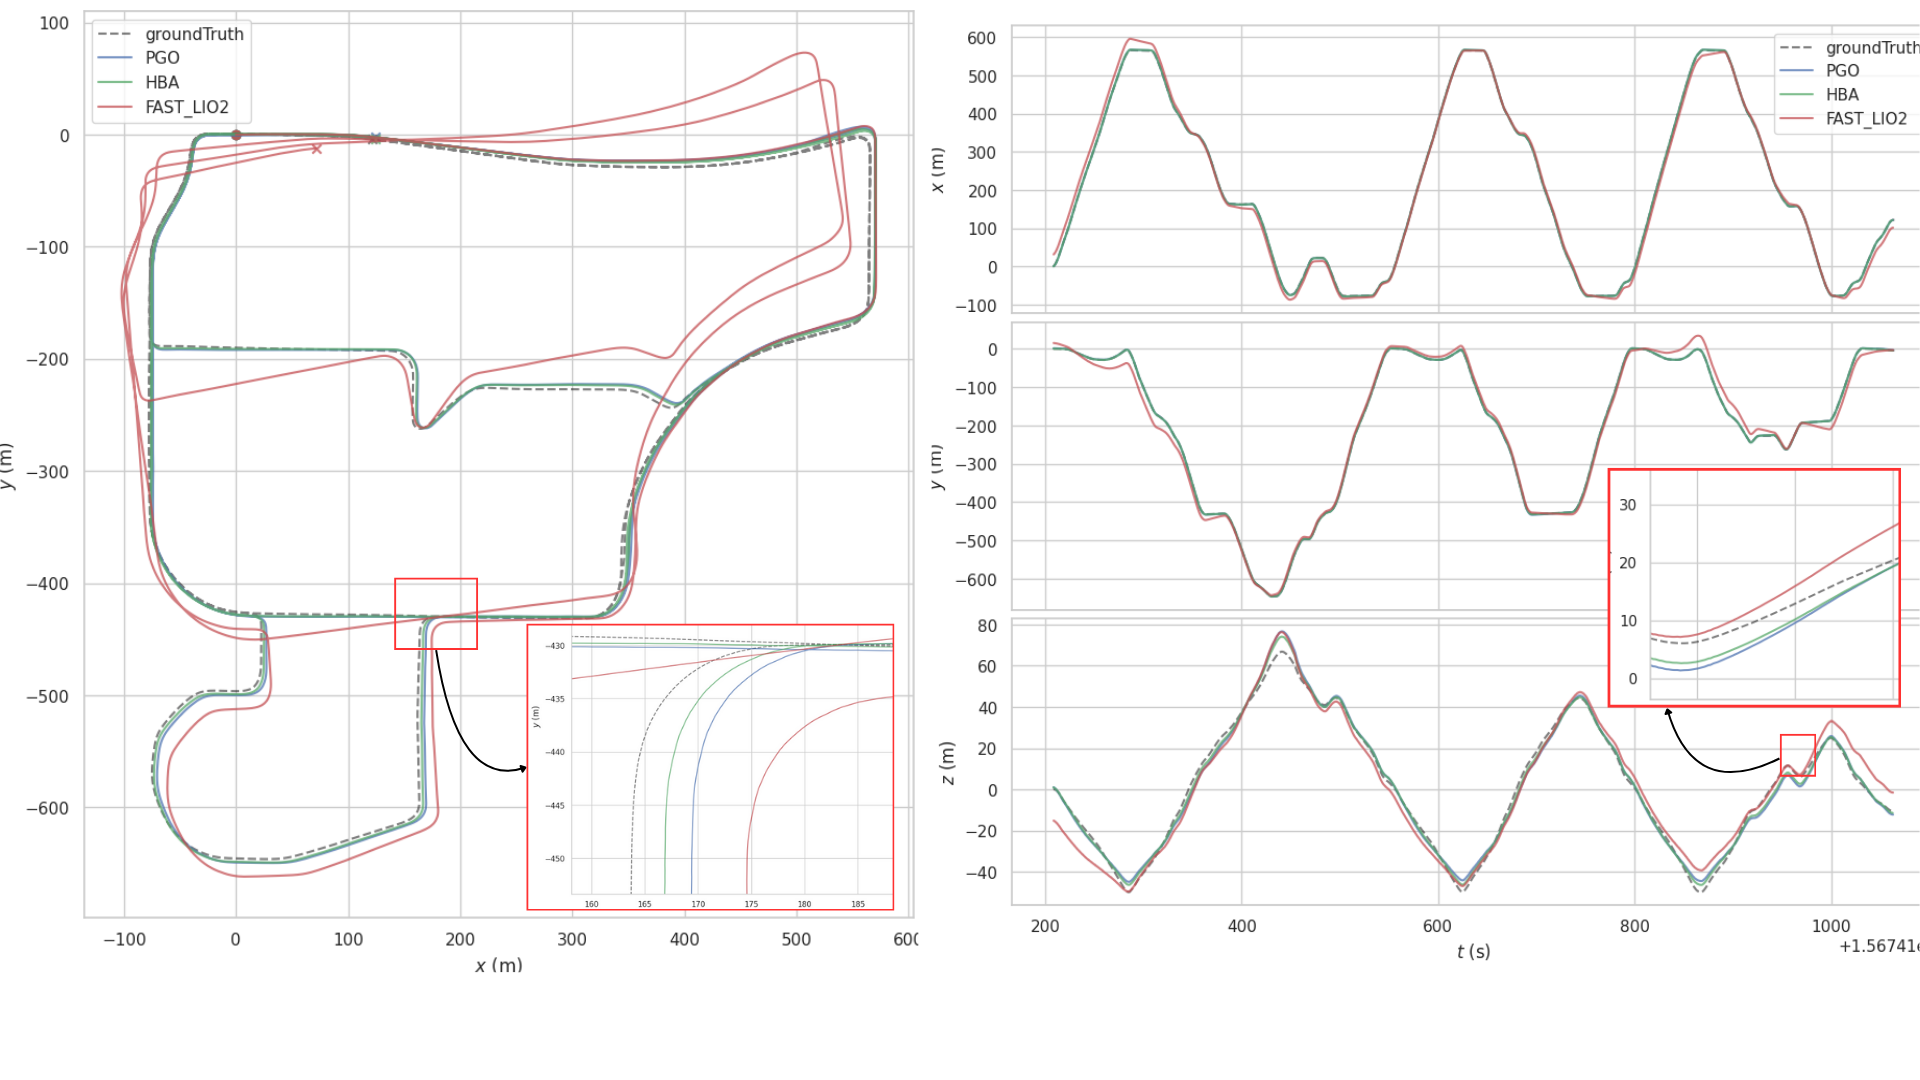
\includegraphics[width=\textwidth]{images/kaist03_trajectory.png}
%	\caption{Trajectories for MulRan KAIST03 sequence. a) Comparison of FAST-LIO2, PGO, and HBA trajectories with ground truth trajectory. b) Axis-wise comparison}
%	\label{fig:kaist03_traj}
%\end{figure}
\begin{figure}[H]
	\centering
	\begin{subfigure}[b]{0.49\textwidth}
		\centering
		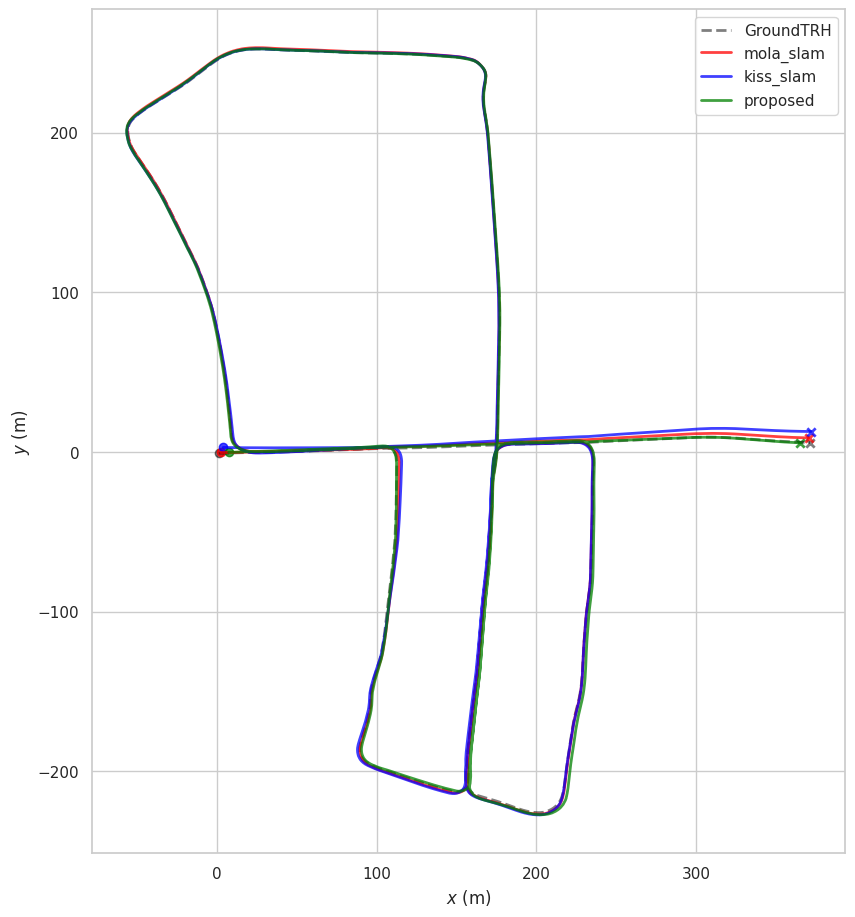
\includegraphics[width=\linewidth]{images/comparison_traj_ki5.png}
		\caption{}
		\label{sub_fig:ki5_traj}
	\end{subfigure}
	\hfill
	\begin{subfigure}[b]{0.49\textwidth}
		\centering
		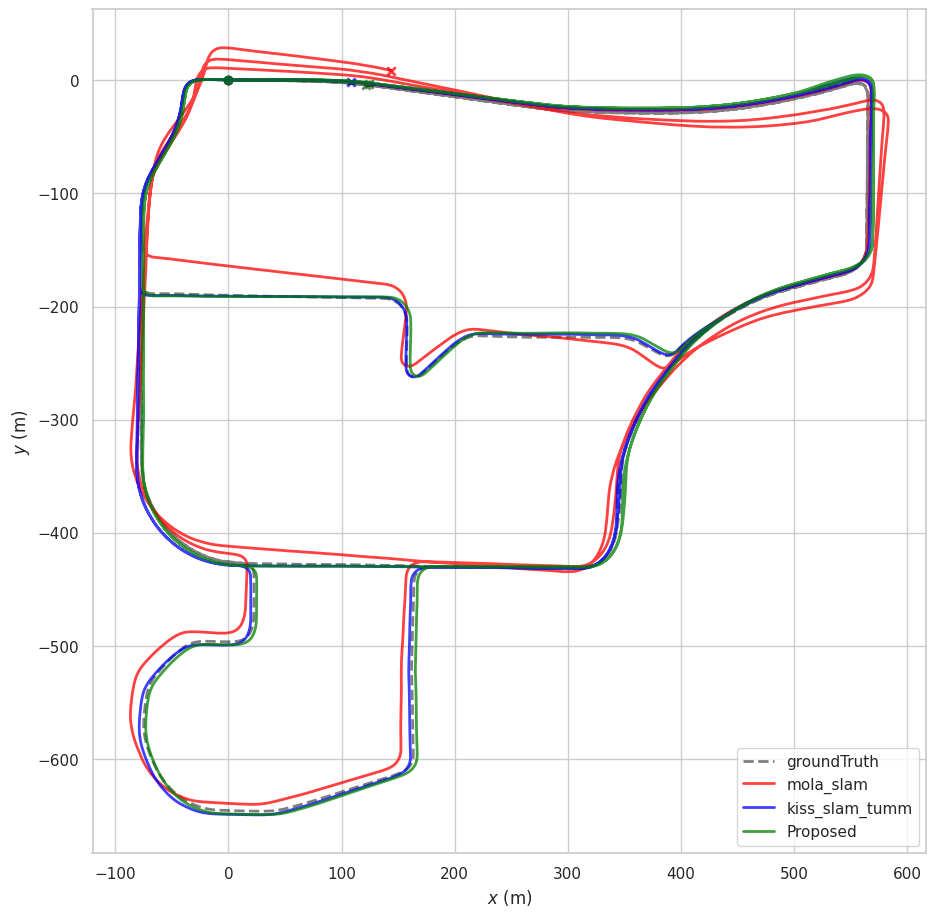
\includegraphics[width=\linewidth]{images/comparison_traj_ka3.png}
		\caption{}
		\label{sub_fig:ka3_traj}
	\end{subfigure}
	\begin{subfigure}[b]{0.49\textwidth}
	\centering
	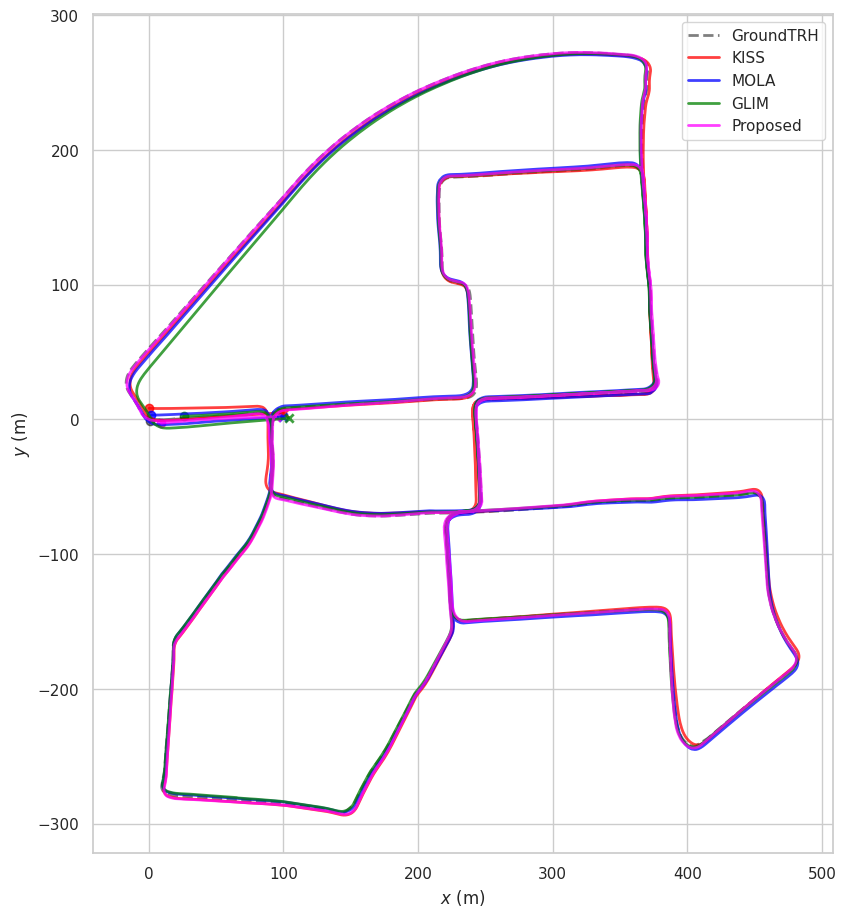
\includegraphics[width=\linewidth]{images/kitti00_traj.png}
	\caption{}
	\label{sub_fig:ki00_traj}
\end{subfigure}
	
	\label{fig:kaist03_traj}
\end{figure}

\begin{figure}[h!]
    \centering
    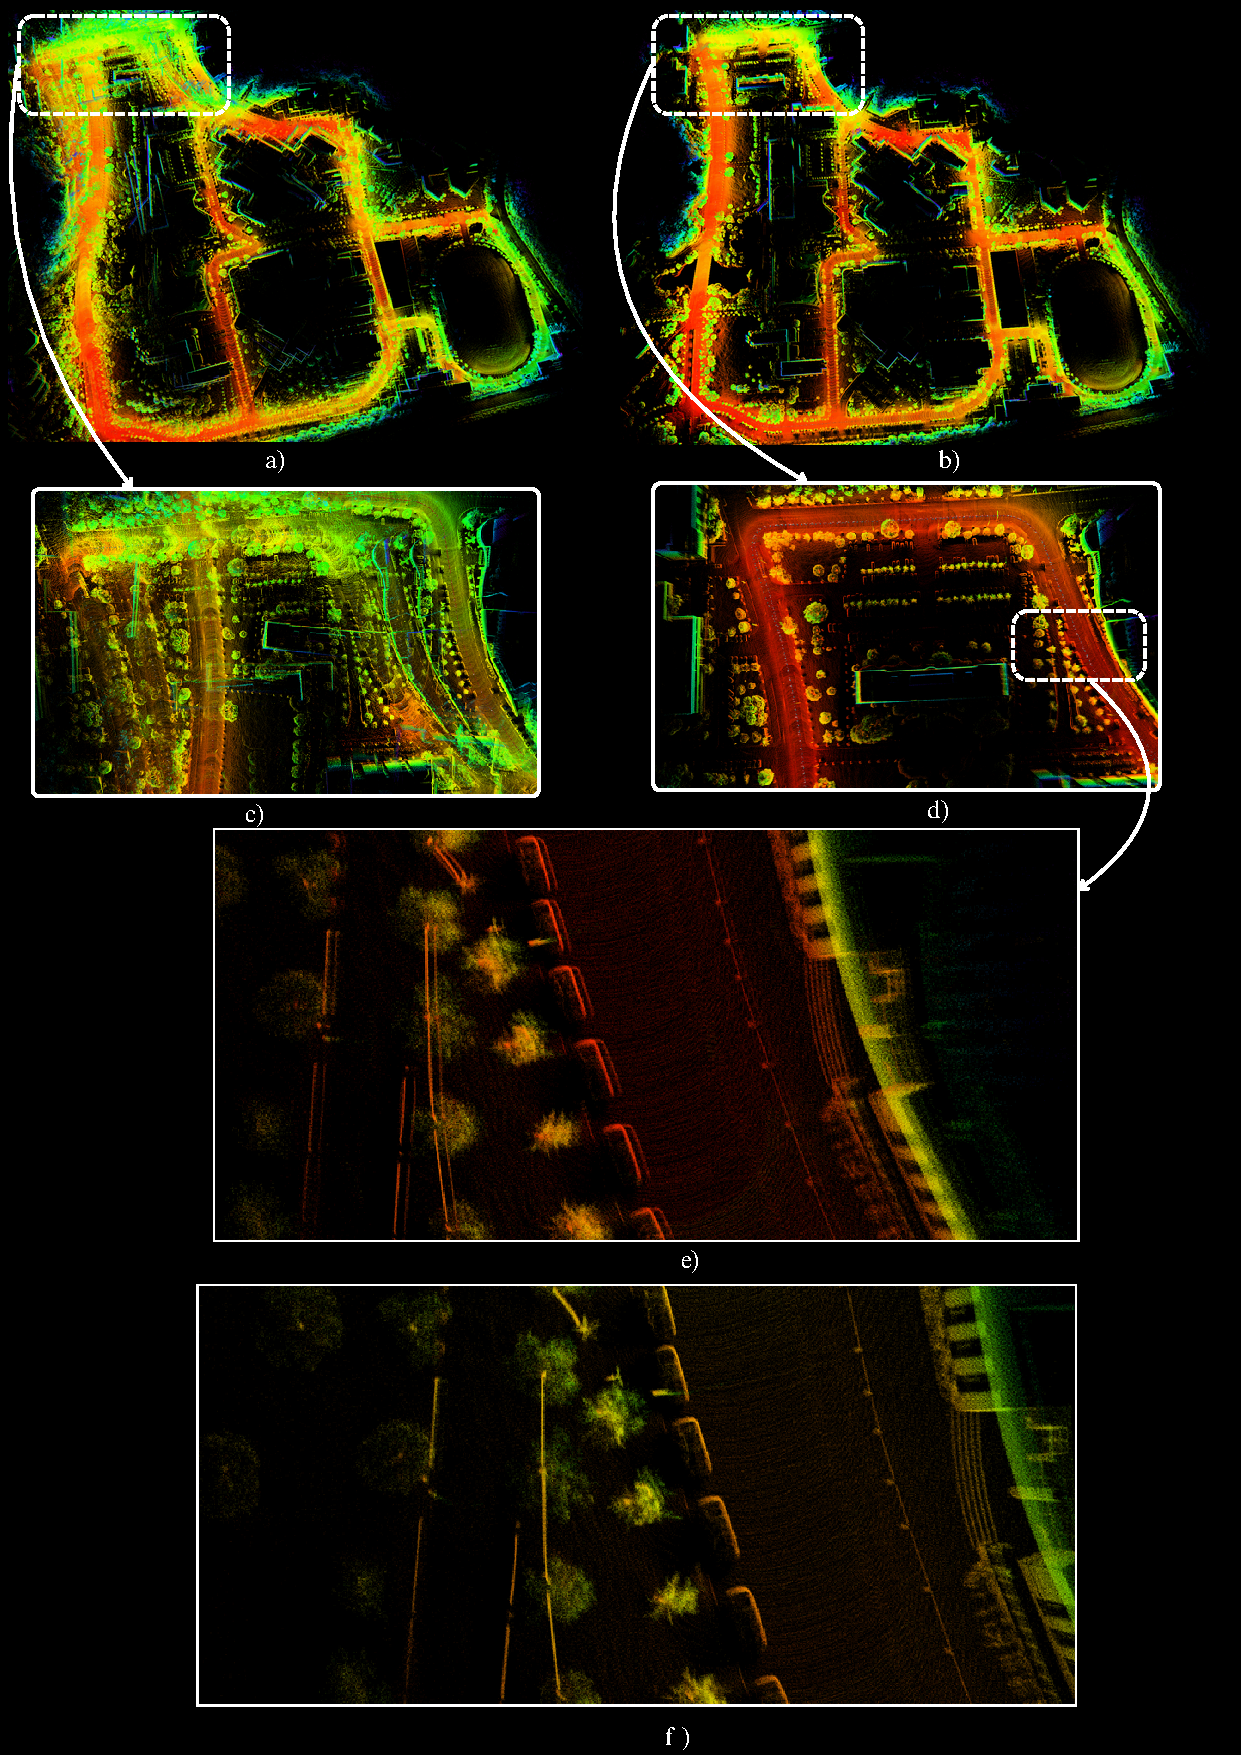
\includegraphics[width=0.9\textwidth]{images/kaist3.pdf}
    \caption{Map generated by each stage of the mapping pipeline for MulRan KAIST dataset sequence 03. \textbf{(a)} Map generated by FAST-LIO2, \textbf{(b)} Map after optimizing with PGO, \textbf{(c)} and \textbf{d)} show segments from \textbf{(a)} and \textbf{(b)} zoomed in respectively. \textbf{(e)} shows the existence of divergence in the map even after PGO. \textbf{(f)} shows the map in \textbf{(e)} after correction with HBA.}
    \label{fig:kaist3_map}
  \end{figure}

\newpage
\section{FAST-LIO2, and PGO map with trajectories for KITTI02}
\begin{figure}[h!]
	\centering
%	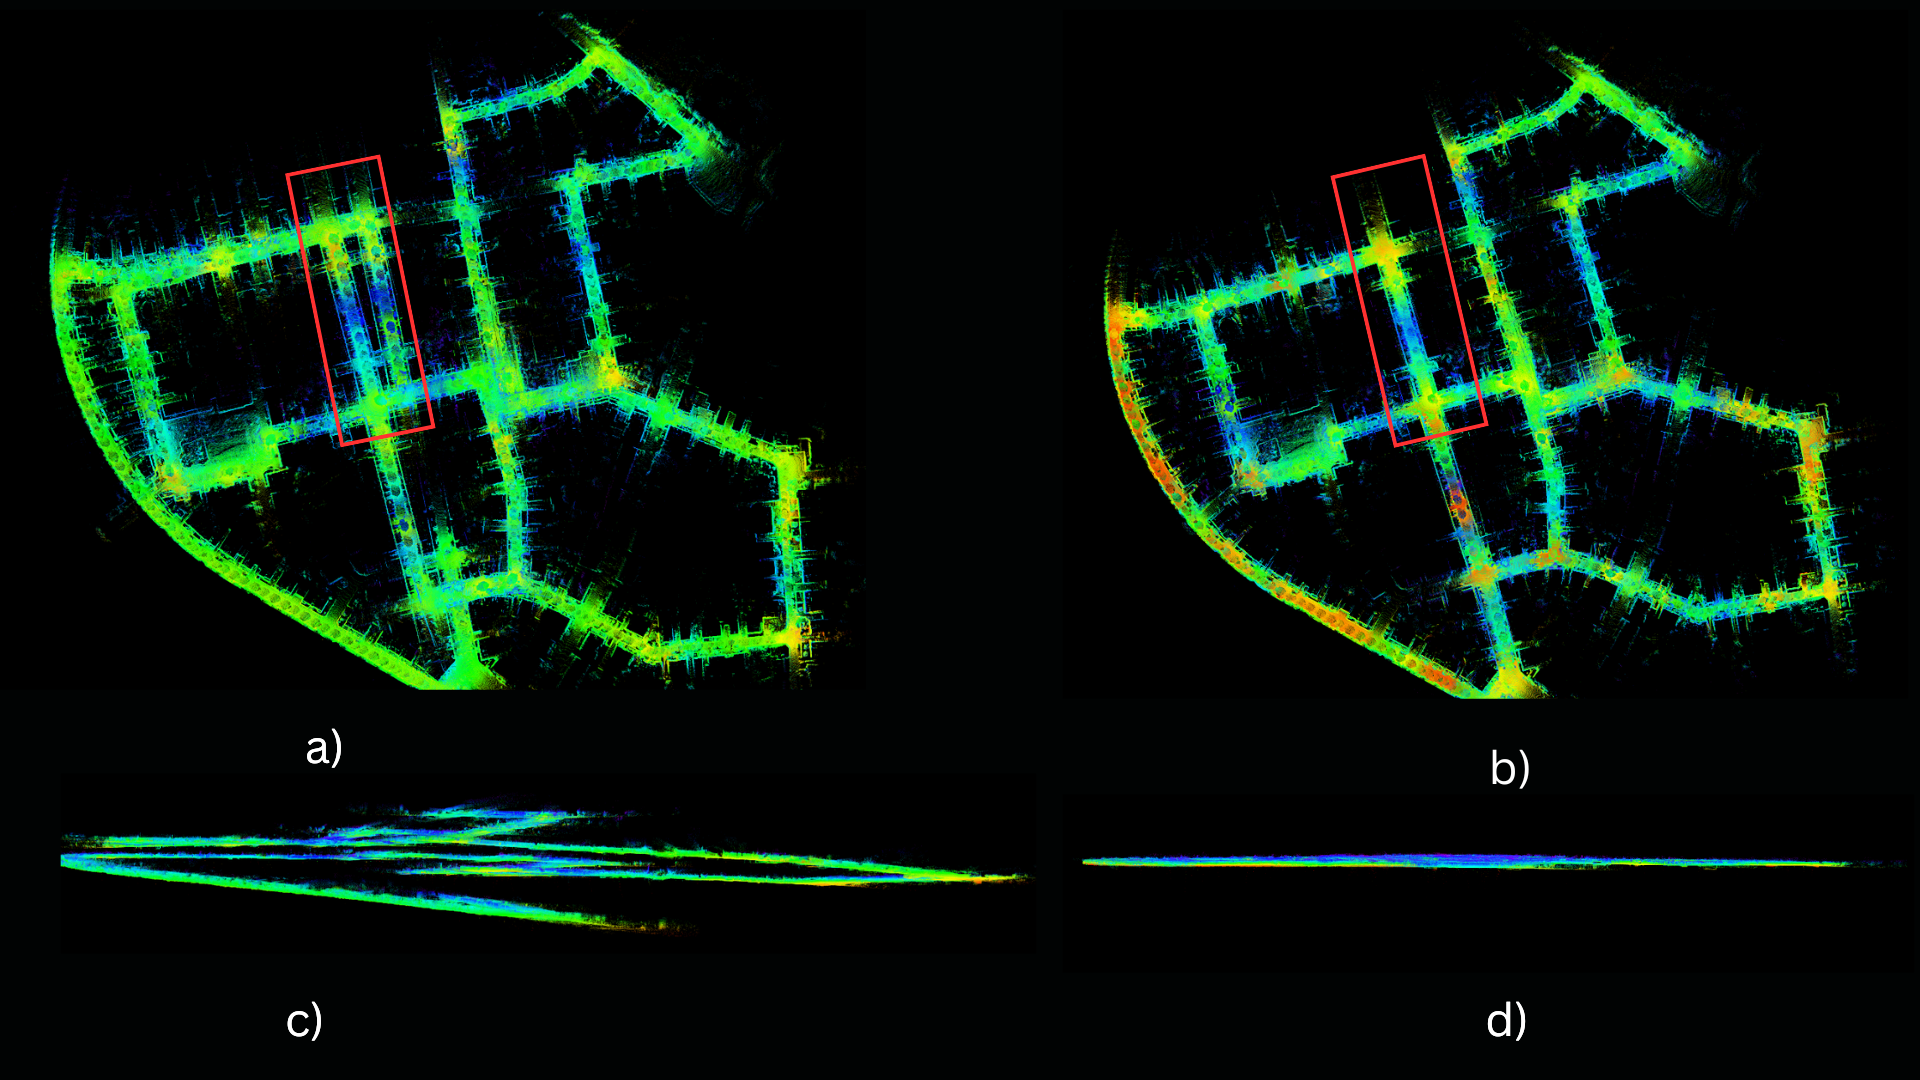
\includegraphics[width=\textwidth]{images/kitti01_odom_pgo_mpa.png}
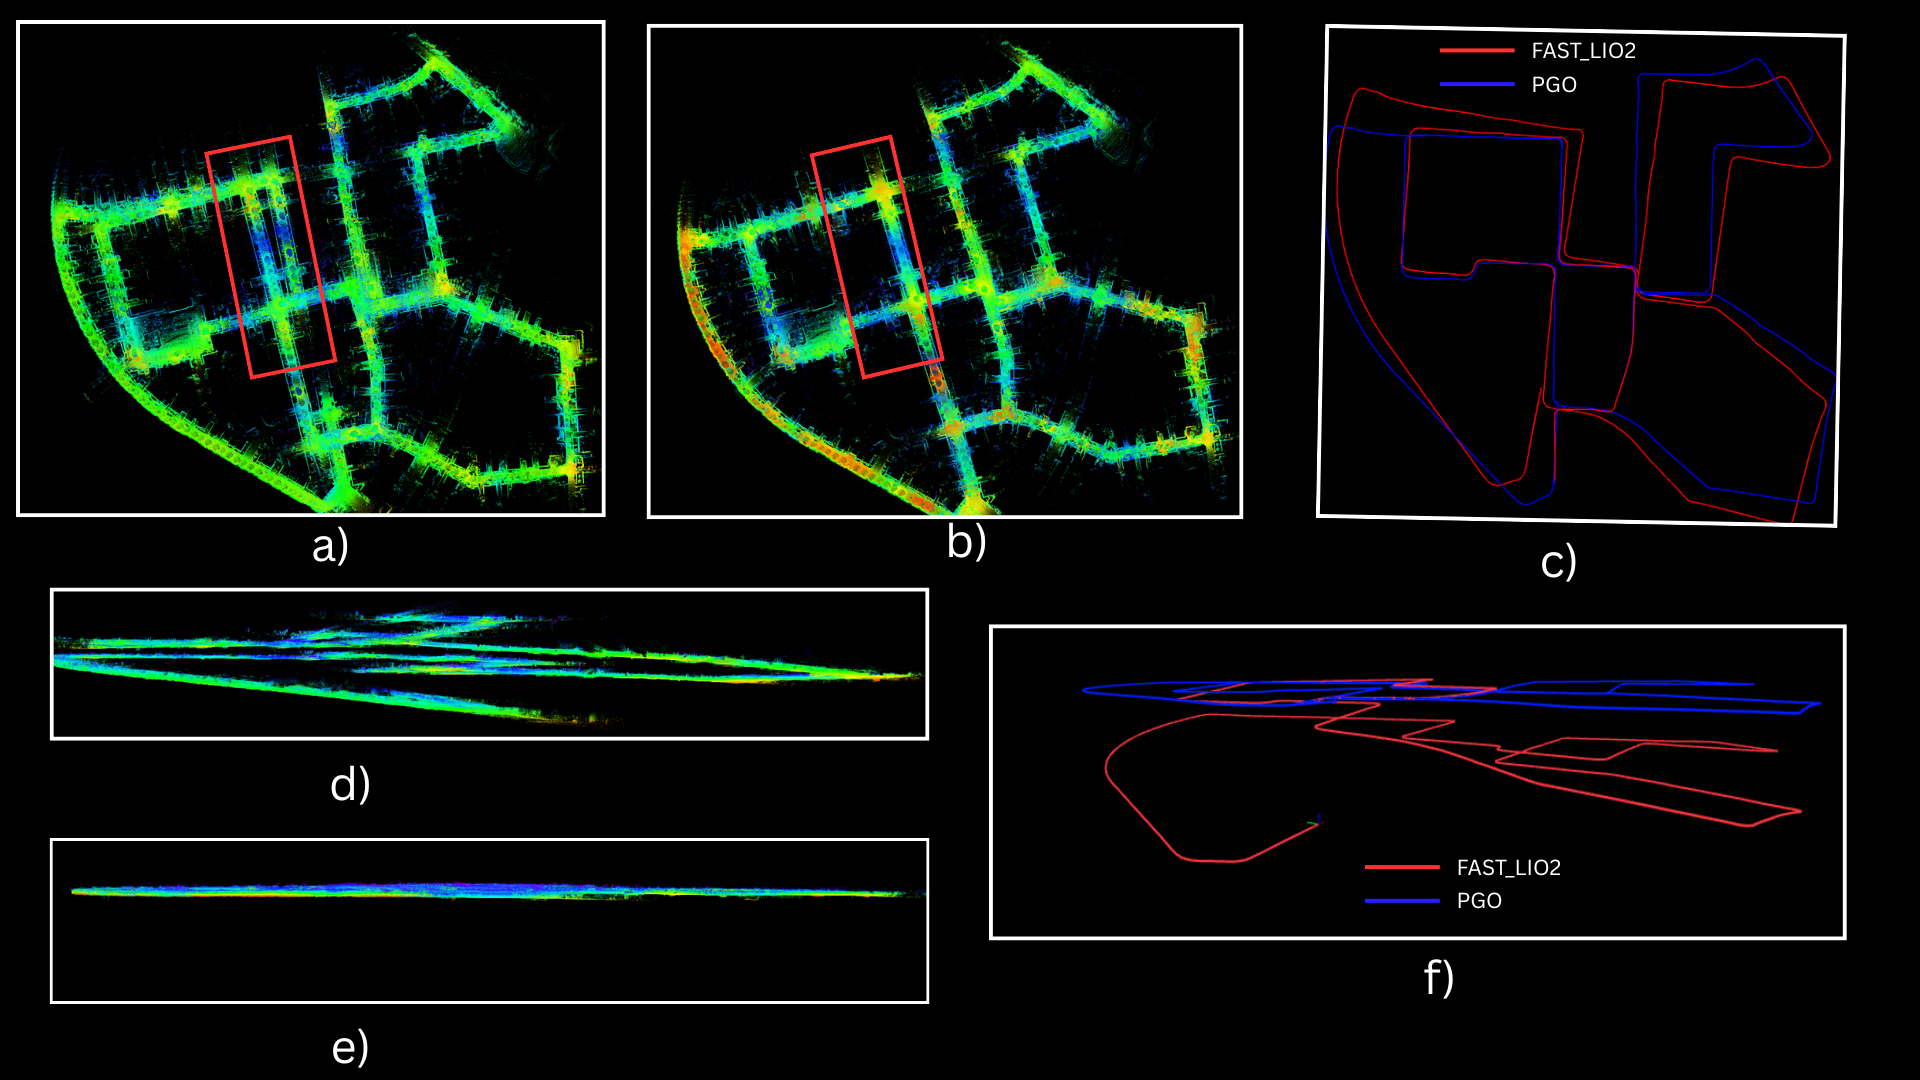
\includegraphics[width=\textwidth]{images/kitti00_map_traj.png}
	\caption{Map visualization for KITTI00 sequence. (a) BEV of map generated by FAST-LIO2. (b) BEV of map after PGO optimization. (c) BEV of FAST-LIO2 and PGO trajectories. (d)Side view of FAST-LIO2 map. (e) Side view the optimized map. (f) Side view of FAST-LIO2 and PGO trajectories}
	\label{fig:kitti00_map_odom_pgo}
\end{figure}
\begin{figure}[h!]
	\centering
	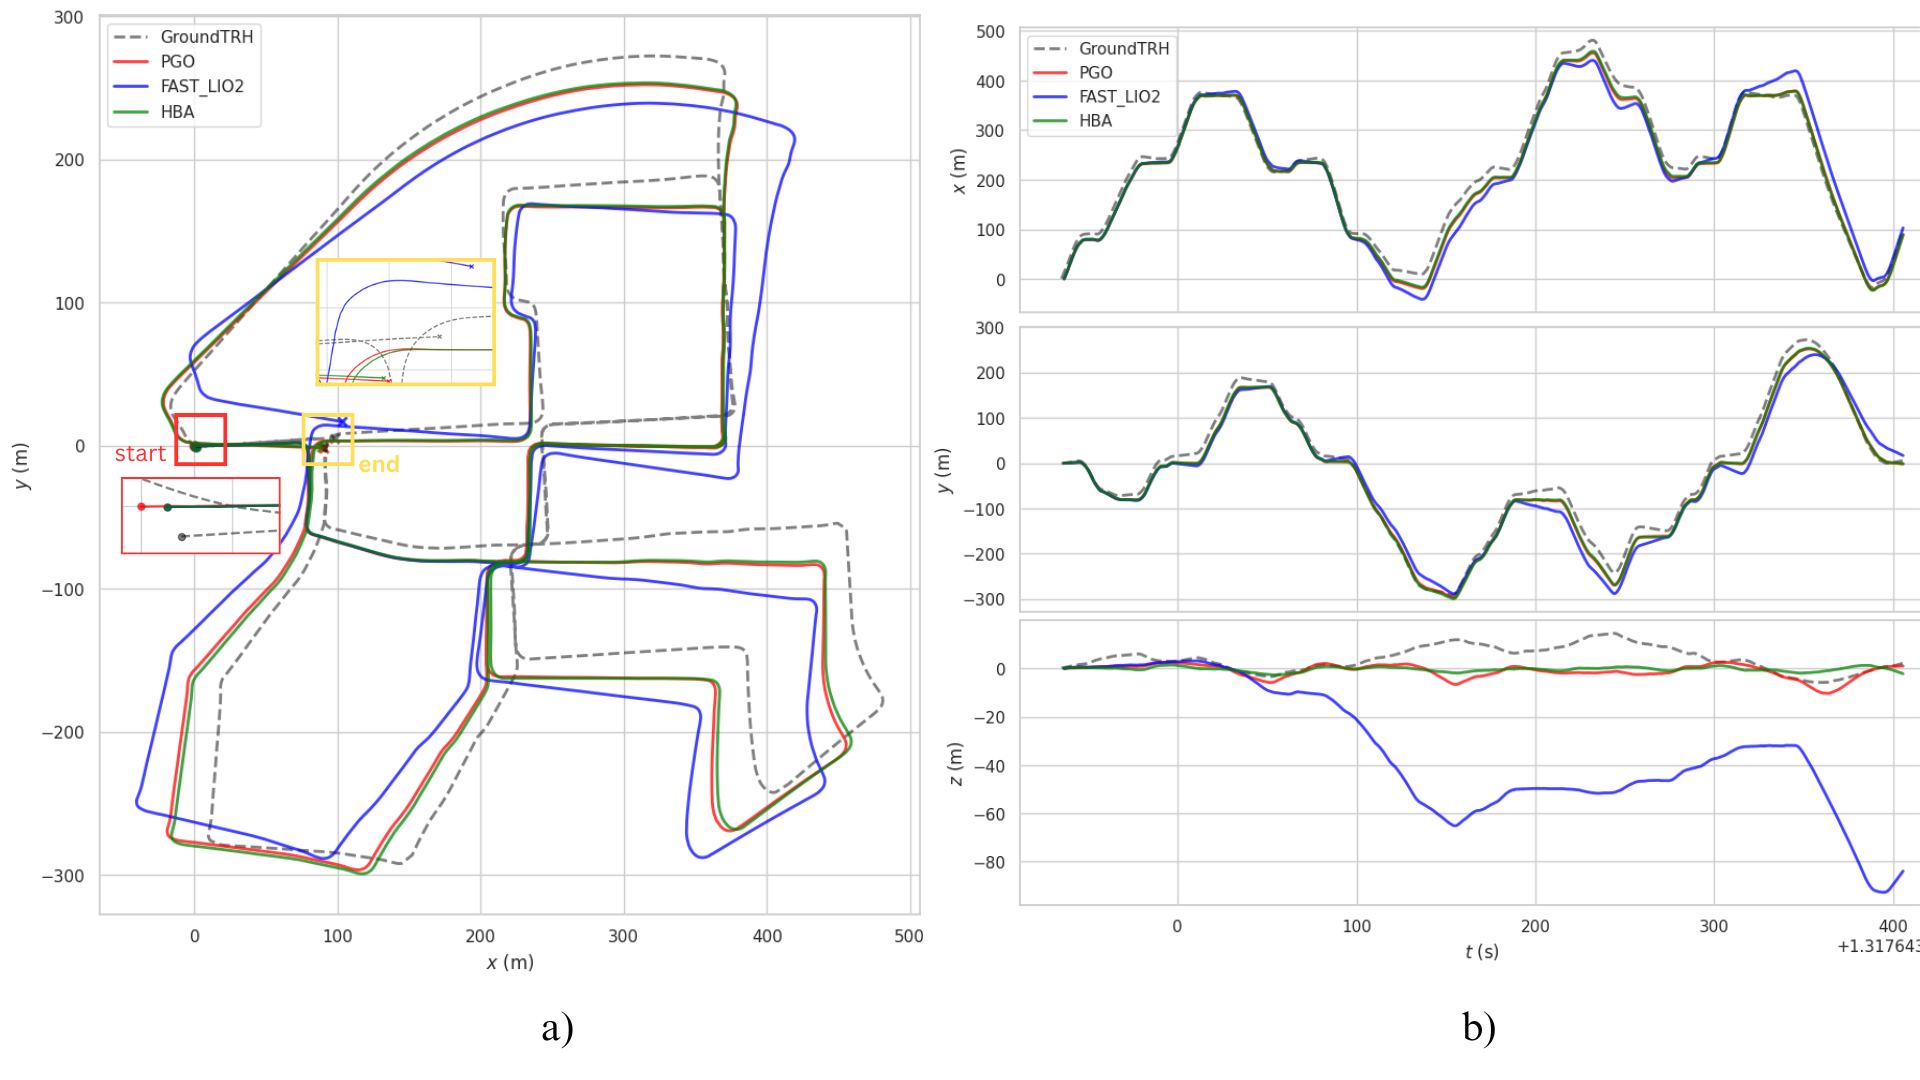
\includegraphics[width=0.9\textwidth]{images/kitti00_trajectory.png}
	\caption{Visualization of trajectories for KITTI00. a) BEV trajectories . b)Axis-wise comparison of the trajectories.}
	\label{fig:kitti00_traj_odom__pgo}
\end{figure}

\section{Results for Saxion11(Indoor)}
\begin{figure}[H]
	\centering
	\begin{subfigure}[b]{0.49\textwidth}
		\centering
		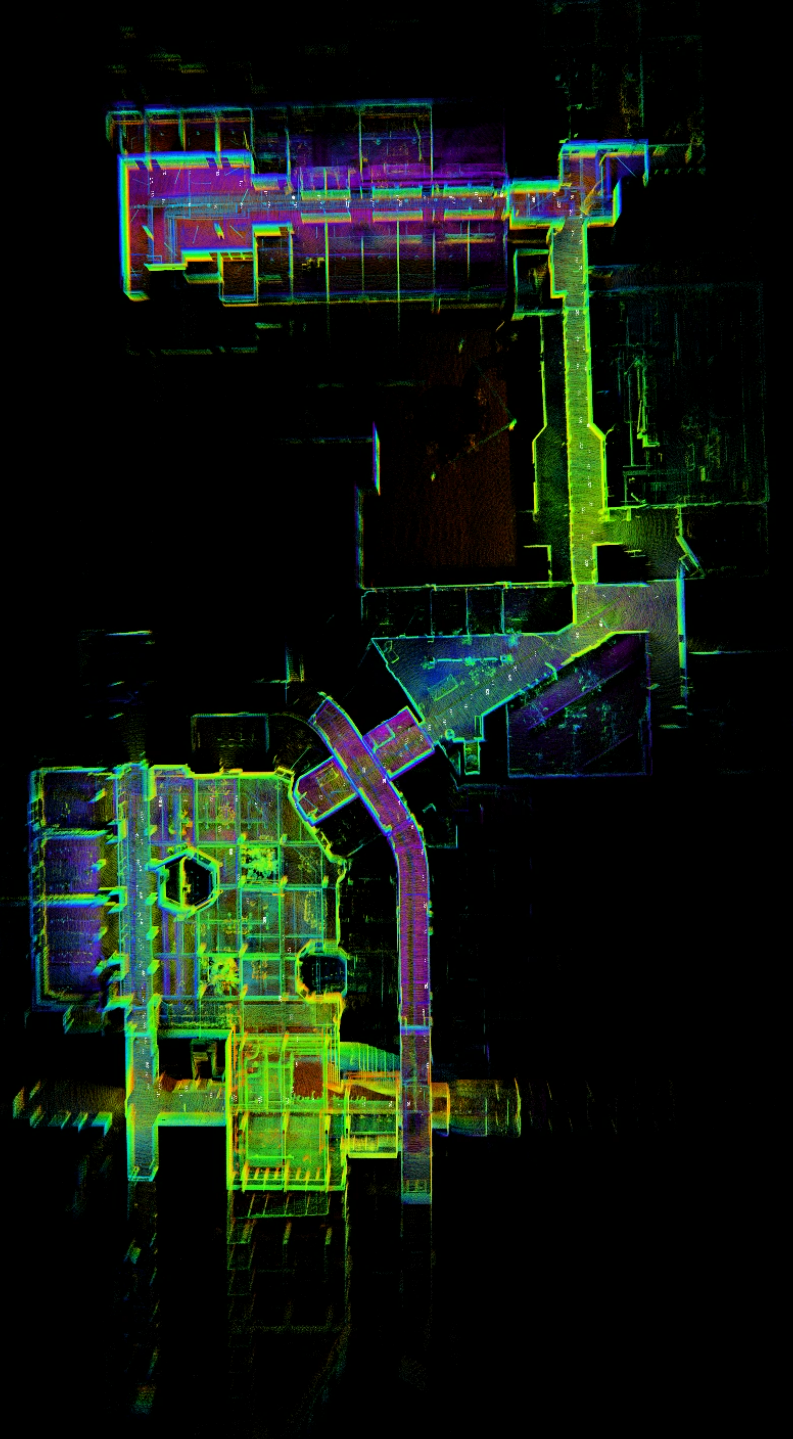
\includegraphics[width=\linewidth]{images/indoor_map.png}
	\end{subfigure}
	\hfill
	\begin{subfigure}[b]{0.49\textwidth}
		\centering
		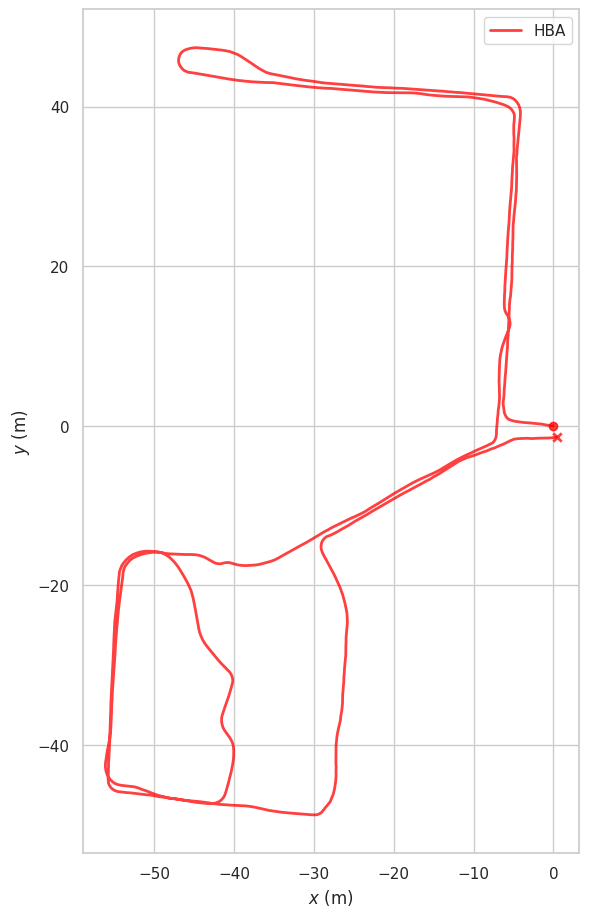
\includegraphics[width=\linewidth]{images/indoor_traj.png}
		
	\end{subfigure}
	\caption{Mapping result for \texttt{saxion11}[Indoor]}
	\label{fig:saxion_indoor}
\end{figure}

\section{ROS node structure}